\begin{figure*}[t]
\centering
\resizebox{0.92\textwidth}{!}{%
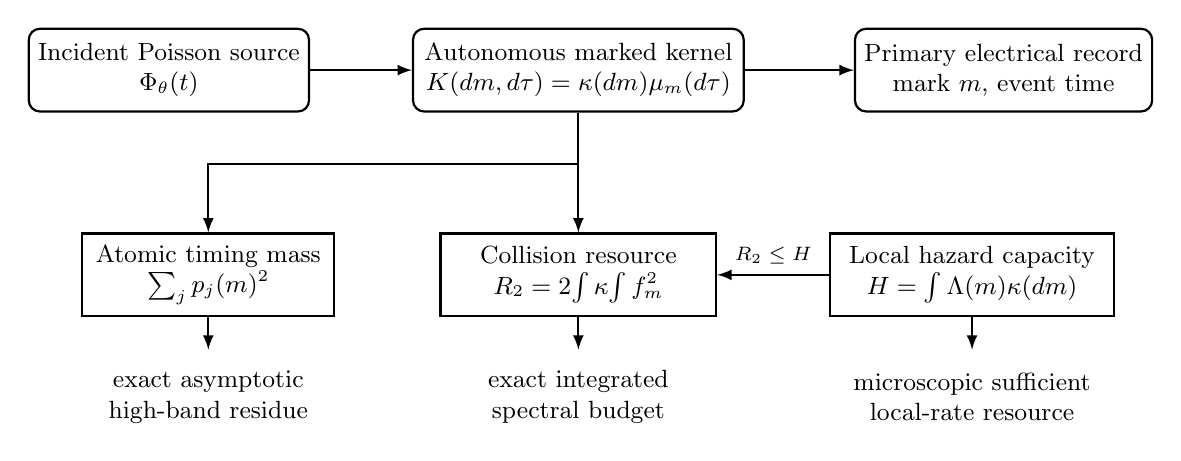
\begin{tikzpicture}[>=latex, line width=0.8pt, font=\small]
  \node[draw, rounded corners, minimum width=3.4cm, minimum height=1.05cm, align=center] (src) at (0,0)
    {Incident Poisson source\\$\Phi_\theta(t)$};
  \node[draw, rounded corners, minimum width=4.2cm, minimum height=1.05cm, align=center] (ker) at (5.2,0)
    {Autonomous marked kernel\\$K(dm,d\tau)=\kappa(dm)\mu_m(d\tau)$};
  \node[draw, rounded corners, minimum width=3.7cm, minimum height=1.05cm, align=center] (rec) at (10.6,0)
    {Primary electrical record\\mark $m$, event time};

  \draw[->] (src) -- (ker);
  \draw[->] (ker) -- (rec);

  \node[draw, minimum width=3.2cm, minimum height=1.05cm, align=center] (atom) at (0.5,-2.6)
    {Atomic timing mass\\$\sum_j p_j(m)^2$};
  \node[draw, minimum width=3.5cm, minimum height=1.05cm, align=center] (r2) at (5.2,-2.6)
    {Collision resource\\$\mathfrak R_2=2\!\int\kappa\!\int f_m^2$};
  \node[draw, minimum width=3.6cm, minimum height=1.05cm, align=center] (haz) at (10.2,-2.6)
    {Local hazard capacity\\$\mathfrak H=\int\Lambda(m)\kappa(dm)$};

  \draw[->] (ker.south) -- ++(0,-0.65) -| (atom.north);
  \draw[->] (ker.south) -- (r2.north);
  \draw[->] (haz.west) -- node[midway,above,font=\scriptsize] {$\mathfrak R_2\le\mathfrak H$} (r2.east);

  \node[align=center] at (0.5,-4.15)
    {exact asymptotic\\high-band residue};
  \node[align=center] at (5.2,-4.15)
    {exact integrated\\spectral budget};
  \node[align=center] at (10.2,-4.15)
    {microscopic sufficient\\local-rate resource};

  \draw[->] (atom.south) -- (0.5,-3.55);
  \draw[->] (r2.south) -- (5.2,-3.55);
  \draw[->] (haz.south) -- (10.2,-3.55);
\end{tikzpicture}%
}
\caption{Resource hierarchy for the autonomous marked-event theorem. The per-photon kernel maps an incident photon into a primary electrical mark and registration delay. Atomic timing mass controls the exact asymptotic flat-band residue; the capture-weighted collision intensity $\mathfrak R_2$ fixes the integrated transfer spectrum; and a capture-weighted local hazard capacity $\mathfrak H$ supplies a microscopic sufficient bound. Source-synchronous clock/control resources are treated separately because they lie outside the autonomous theorem.}
\label{fig:resourceHierarchy}
\end{figure*}
